\DiaryEntry{Probability of the Union of Events}{2015-07-21}{Stochastic}


Based on
\href{https://terrytao.wordpress.com/2010/01/01/254a-notes-0-a-review-\%20\%5Bof-probability-theory/}{Exercise
15} in Terry Tao's blog.

Two events $E_1, E_2$ with probabilites $P(E_1) = P_1, P(E_2) = P_2$. Below we assume independent events; that is $P(E_1, E_2) = P(E_1) \times P(E_2)$; or, to be more exact $P(E_1=e_1 \cap E_2=e_2) = P(E_1=e_1) \times P(E_2=e_2)$.

\begin{figure}[hbt!]
\centering
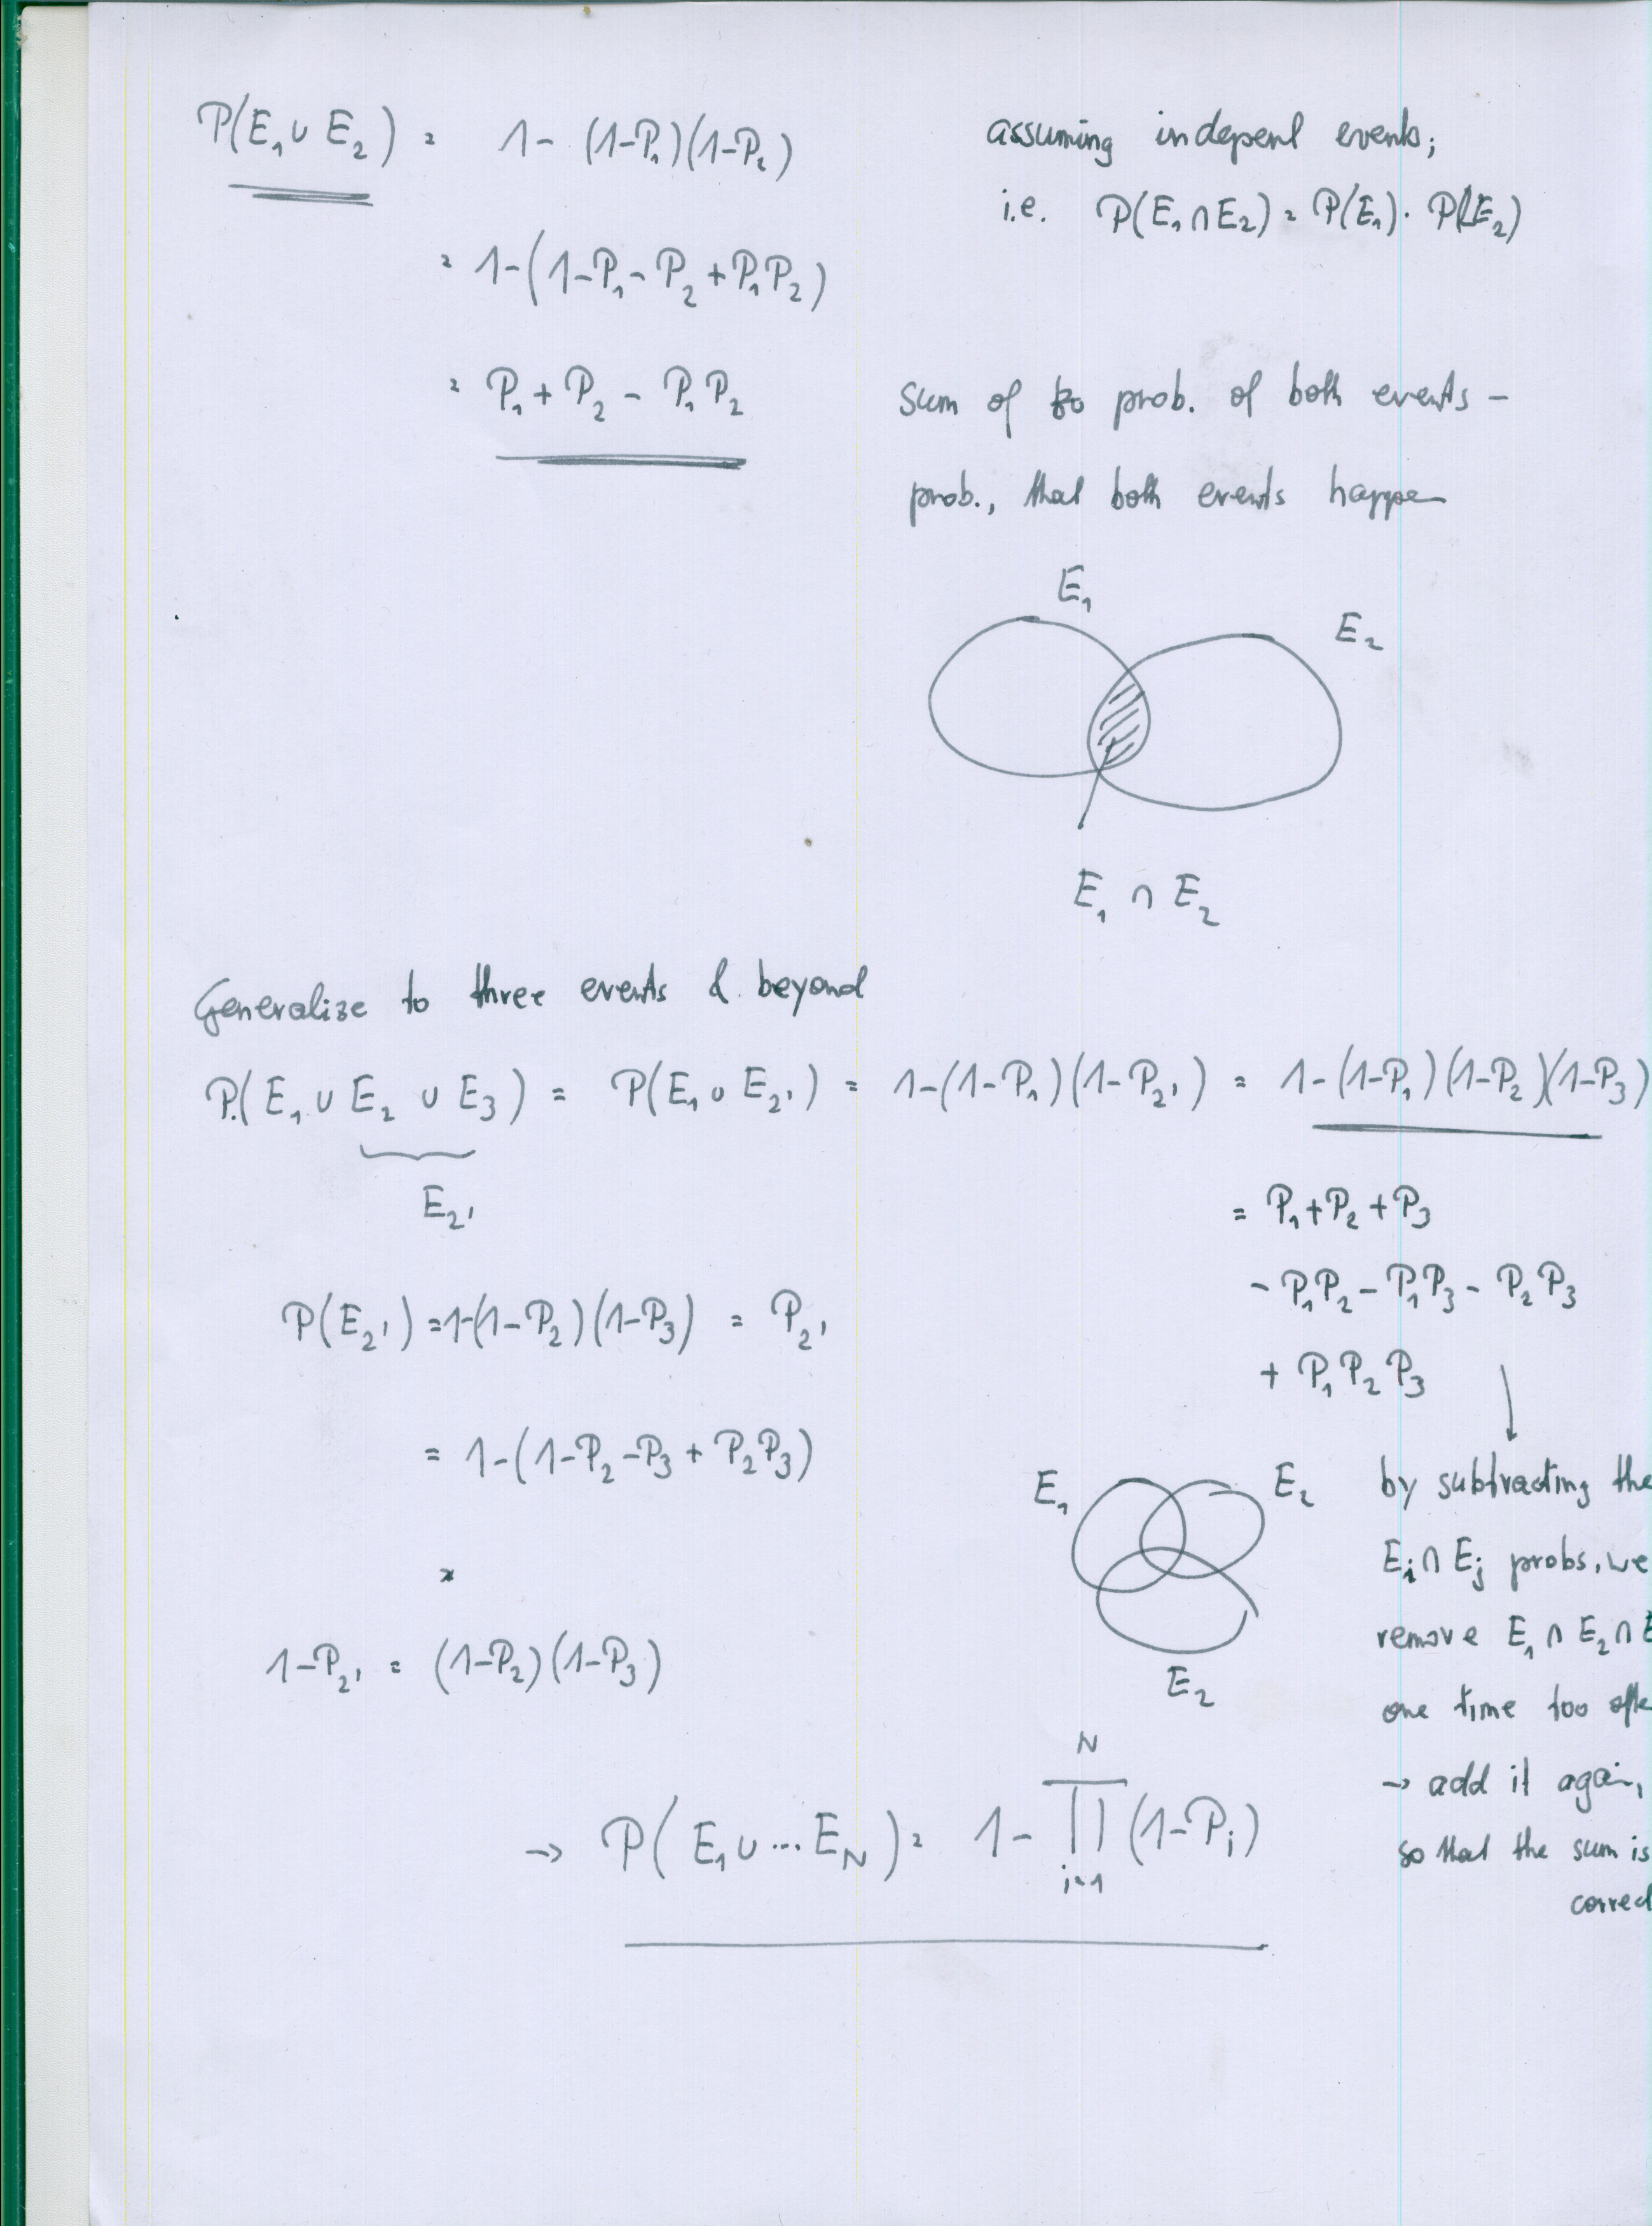
\includegraphics[scale=0.5]{images/union_probability.png}
\caption{Page1}
\end{figure}

Similar (probability is proportional to the size of sets), there is the Sieve Formula for calculating the size of the union of sets:

\[ |A_1 \cup A_2 \cup \cdots A_n| = \sum_{j=1}^n (-1)^{j-i} \sum_{i_1, i_2, i_j} | A_{i_1} \cap A_{i_2} \cap \cdots A_{i_j}|\]

where $i_1, i_2, \ldots , i_j$ covers all j-element subsets of $[n]$.

For the case $n=2$, we therefore have

\[ |A_1 \cup A_2| = |A_1| + |A_2| - |A_1 \cap A_2| \]

for $n=3$, we have

\[ |A_1 \cup A_2 \cup A_3 | = |A_1| + |A_2| + |A_3| - |A_1 \cap A_2| - |A_1 \cap A_3| - |A_2 \cap A_3| + |A_1 \cap A_2 \cap A_3| \].

Compare this with the results in the handwritten notes above.
